\documentclass[twoside,11pt]{article}

% Any additional packages needed should be included after jmlr2e.
% Note that jmlr2e.sty includes epsfig, amssymb, natbib and graphicx,
% and defines many common macros, such as 'proof' and 'example'.
%
% It also sets the bibliographystyle to plainnat; for more information on
% natbib citation styles, see the natbib documentation, a copy of which
% is archived at http://www.jmlr.org/format/natbib.pdf

\usepackage{jmlr2e}
\usepackage{graphicx}
\usepackage{amsmath}
\graphicspath{ {images/} }



\begin{document}

\title{Research Paper: Machine Learning Application for Brain Tumor Localization in the  Repository of Molecular Brain Neoplasia Data (REMBRANDT) }

\maketitle
\textbf{Machine Learning for Health Care (Heinz 95-845) - Lukas Mohs}


\section{Abstract}
\noindent Within this paper, I want to present the putcome of the  combined application of \textit{Computer Vision} (CV) and  \textit{Machine Learning} (ML) to the \textit{Repository of Molecular Brain Neoplasia Data } (REMBRANDT) dataset. This dataset contains pre-surgical \textit{magnetic resonance} (MR) multi-sequence images of 130 patients. Based on a visual analysis and the application of several ML algorithms, I tried to predict the location of the brain tumor and compare it to the evaluation of three Radiologist, which defined the affected brain part and the potential impact on the brain functionality.i

\section{Introduction and Background}
\subsection{Brain Cancer}
Among all types of cancer, brain cancer is one of the deadliest even if it's not one of the most common ones. With a so-called \textit{5-Year Relative Survival Rate} of 32 \% for white people and 39 \% for black people it ranks on place 7 out of 26 for the lowest survival rate. Specific cancer types like \textit{Glioblastoma}, a very fast growing type of tumor, even has a a rate of 5\%. Especially in the later years of life, this rate decreases heavily for all types of brain cancer. \citep{cite1}
The high variance in the surivial rate is given by many factors such as the type of tumor, the location and of course whether it was treated. Especially the latter ones formed a major part of scientific studies that included ways of scanning the human brain for malignant tissue as well as the way of stopping the growth of the tumor cells. \citep{cite2}


\subsection{Magnetic Resonance Imaging (MRI)}
\textit{Magnetic Resonance Imaging} (MRI) addressed the challange of 
\textit{scanning} the human body by using \textit{radiology}  to see different layers of the inner tissue or organs. These different layers can be combined together to construct a 3-dimensional model of any part of the body. Mainly a strong  \textit{magnetic fields} is used in combination with \textit{radio waves}  and so-called \textit{field gradients}.
In comparison to \textit{Computer Tomography} (CT), MRI doesn't rely on \textit{X-radiation}, which qualifies it as a less harmful method. It should be mentioned that the magnetic waves of MRI can affect \textit{cardiac pacemakers} so that exceptions apply. \citep{edelman1993magnetic}

\subsection{The Human Brain}
Especially the development and refinement of the MRI technology favored advanced studies about the structure and functionality of the human brain. In order to understand the classification task of the presented algorithm, the major parts of the human brain are shortly described and visualized in Figure \ref{fig:brain}:
\begin{figure}
	\centering
	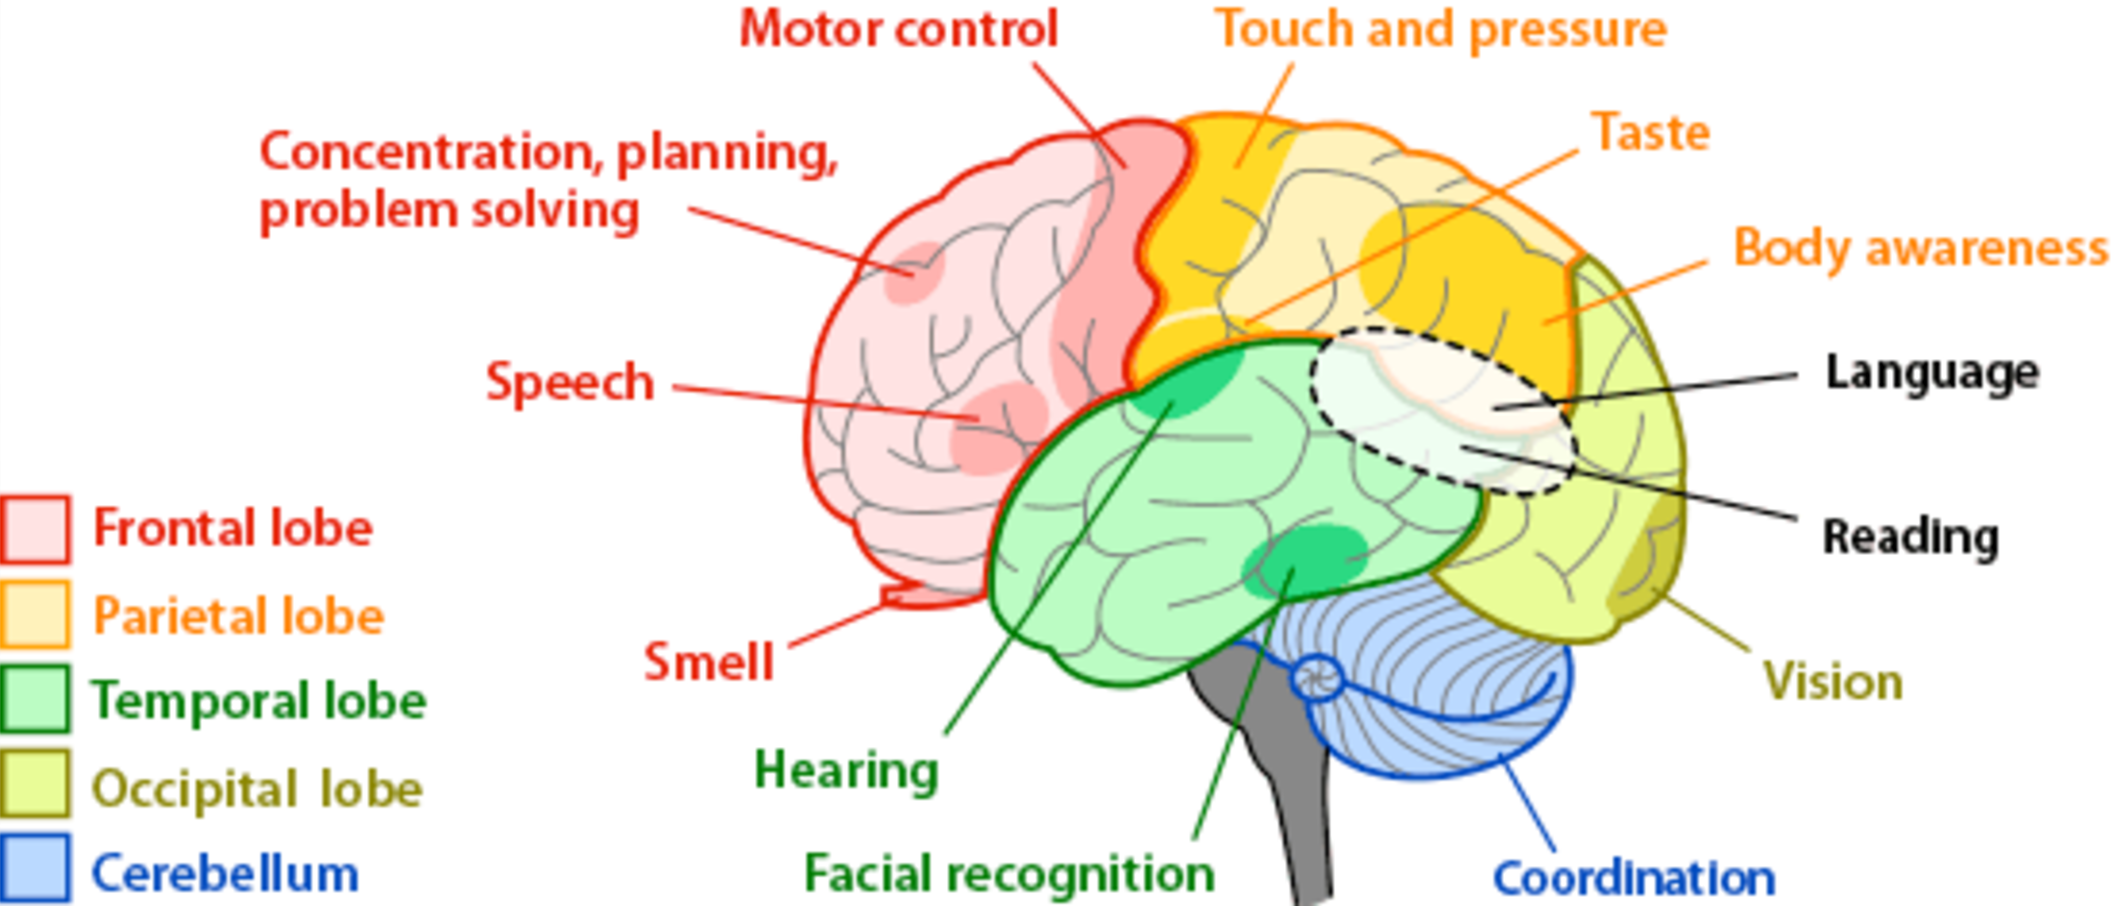
\includegraphics[width=10cm]{brain-areas}
	\label{fig:brain}
	\caption{Brain Areas (source: Arizona State University)}
\end{figure}%

\begin{itemize}
	\item \textit{Frontal Lobe:} resides in the front of the head and is the only lobe on the lateral surface and separated from the other ones. It is responsible for problem solving, planning but also processes stimuli from the nose. 
	\item \textit{Temporal Lobe:} caudally joins the parietal and occipital lobe without a clear boundary. Researchers could show that it hosts the function of recognizing faces.
	\item \textit{Parietal Lobe:} is Clear separated from frontal lobe but merges into temporal and occipital lobe. It is important for the control of the body including the sense of touch.
	\item \textit{Occipital Lobe:} has also no clear coundary to its neighbours (parietal and temporal lobe). The stimuli of the eye are for example processed by this lobe.
	\item \textit{The Insula:} is a small portion of the cerebral cortex and hidden by the other outer lobes. It is believed to be responsible for  consciousness.
	\item \textit{The Cerebellum:} is placed on the back of the head below the occipital lobe and next to the \textit{brain stem}. It could be shown that it is responsible for fine motoric controls and languages.
\end{itemize}
\citep{duvernoy2012human}

\subsection{Computer Vision}
\label{cv}
\textit{Computer Vision} (CV) is a field of \textit{Computer Science} that focusses on the way of how to digitally process, analyze and understand images. Driven by the development of cheap cameras and computing power, CV is applied in many cirsumstances to support or replace the human's richest sense: the eye.
To provide a highlevel understanding of a CV identification or classification approach, one has to consider the digital representation of an image on the computer. This can be decomposed to a two-dimensional matrix, where each entry holds a tupel of three values: the \textit{\textbf{R}ed}, \textit{\textbf{G}reen} and \textit{\textbf{B}lue} (RGB) channel. This tupel identifies how the color of one specific \textit{pixel} is composed. These matrix of pixels is often referred to as \textit{raster graphic}. Figure \ref{fig:pixel} demonstrates this representation for three specific pixels within an image. In comparison to colorful images, \textit{grayscale images} just has a single channel, which indicates the brightness between black (0 \%) and white (100 \%). Most common file types represent the  channel values  in a range between 0 and 255. The brightness of a colorful image is therefore determined by the average of the sum of each pixel's RGB values. The contrast of an image is referring to the variance of the sum of each pixel's RGB values: the higher the difference, the stronger the contrast. These concepts are important to later understand the image processing algorithm.

\begin{figure}
	\centering
	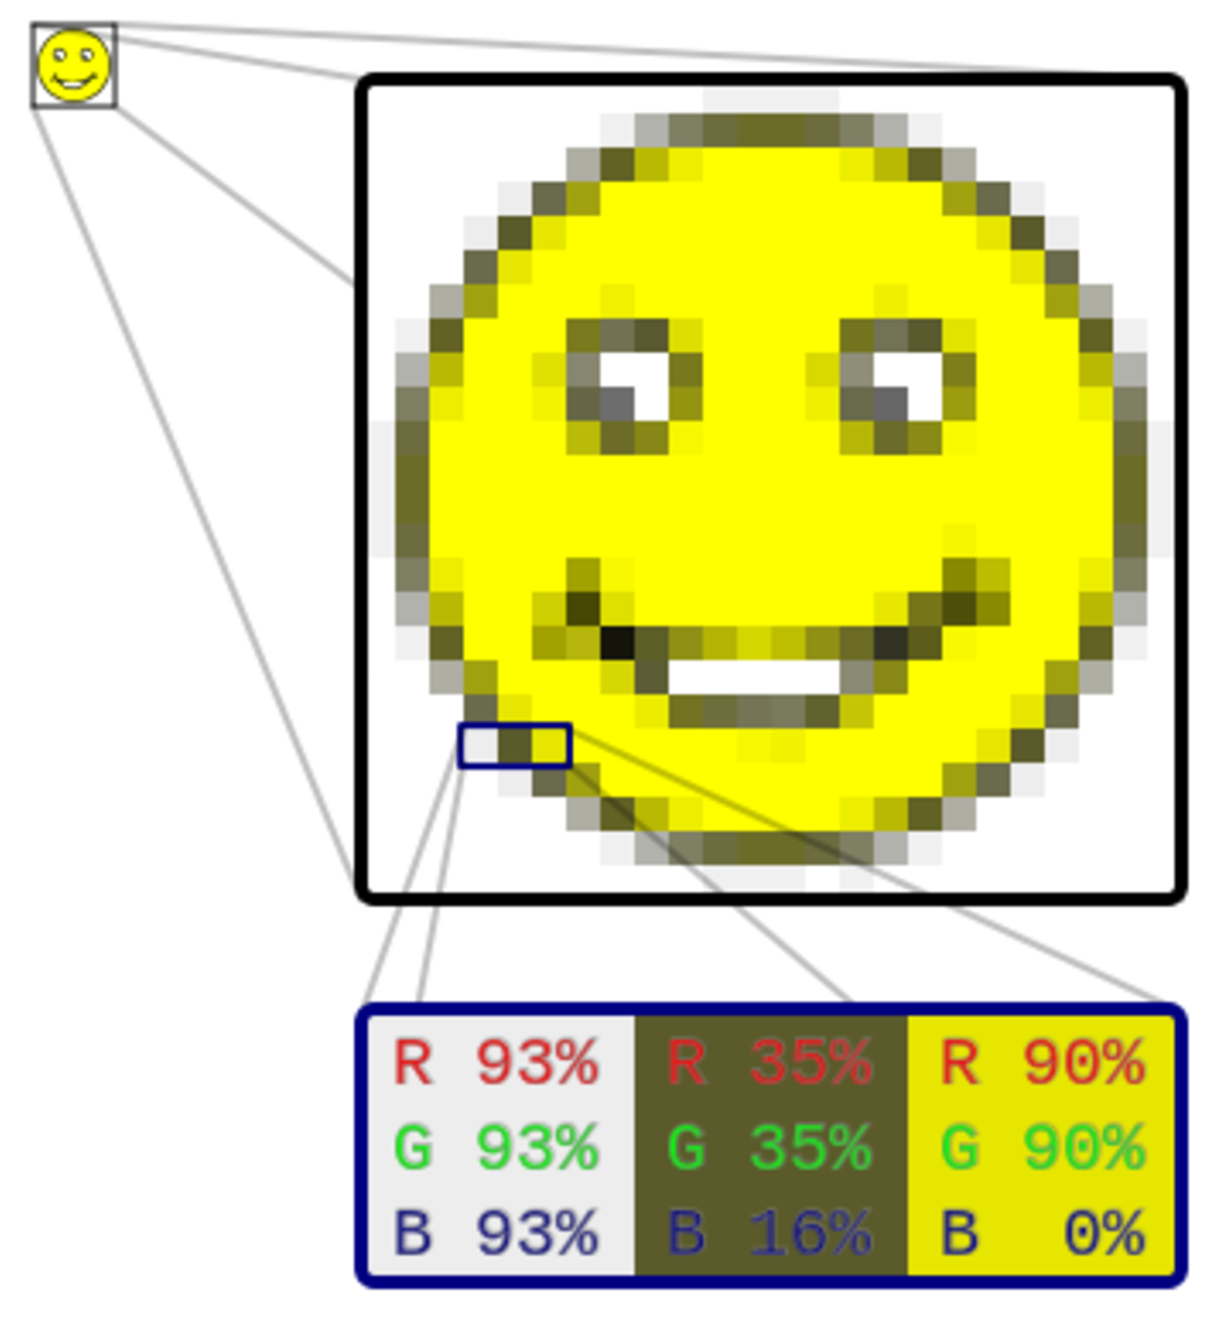
\includegraphics[height=5cm]{pixel}
	\label{fig:pixel}
	\caption{Raster Graphics (source: Wikipedia)}
\end{figure}%

\subsection{Machine Learning}
In the recent years, \textit{Machine Learning} (ML) genereated special attention due to it's successful application in many fields of industry. Generally, ML can be understood as an automized approach of analyzing and learning specific patterns within a big series of data. For this purpose, statistical principles are implemented on a given \textit{training set} afterwards to predict the class or value of new instances. ML is used in this scenario to evaluate the output of the image processing step and locate the brain tumor within a given sequence of MRI scans. In particular, the probabilistic \textit{Naive Bayes} classifier will be used in combination with a \textit{Decision Tree} due to their simplicity, whcih allows a solid interpretabiliby.

\section{Implementation: ML Prediciton based on CV Pattern Matching Outcomes}
Within this section I want to describe the setup and implementation of the \textit{ensemble} of CV and ML that is used to locate the brain tumor within the image sequence retrieved from the MRI scan. Ensemble means that a two-step process is used to realize the final prediction:
\begin{itemize}
	\item First, the images fo the REMBRANDT dataset are retrieved, preprocessed and analyzed by the application of several pattern matching methods.
	\item Then, the output of the analysis is written to \textit{CSV} file to be taken as an input for the ML learning and prediction approach.
\end{itemize}
The most recent version of the source code of this project, which is based on  \textit{Python} for the image processing and \textit{R} for the ML part, can be found on Github: 

\textit{https://github.com/lukasmohs/TumorDetection} .

\subsection{REMBRANDT Image Data Set}
At this point, the input data in form of a series of image sequences is described: 
The data of REMBRANDT was generated through the Glioma Molecular Diagnostic Initiative and contains the pre-surgical MR multi-sequence images from 130 patients. This image dataset is enriched by a professional classification of three differen radiologists for each individual stating the tumor location within the brain. Each sequence can be defined as one specifc direction of slicing, which was used in order to scan the patient's head. This means that each patient was scanned either  horizontally or vertically from different angles. In figure \ref{fig:sequences}, one image of each of these sequnces for one patient is provided. \citep{cite3}

\begin{figure}
	\label{fig:sequences}
	\centering
	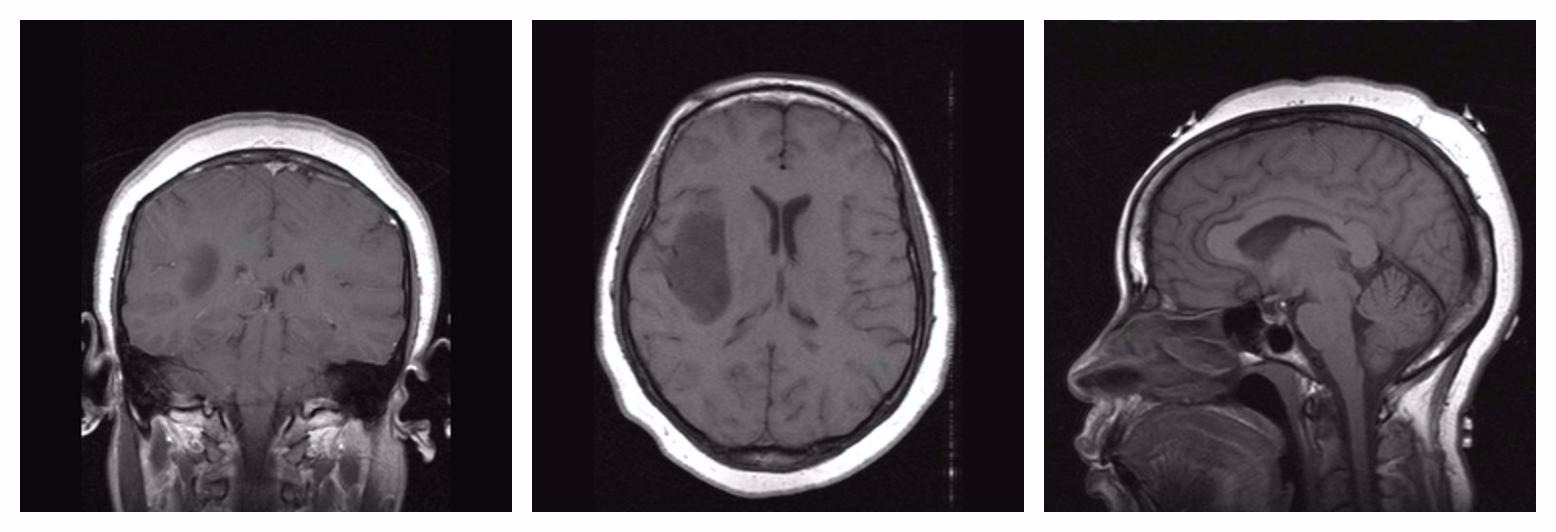
\includegraphics[height=5cm]{sequences}
	\caption{Sequence Comparison (back to front, top to bottom, left to right)}
\end{figure}%

Comparing the images provided from each sequence, we can see that the image on the left  (\textit{back to front}) and the one on the right (\textit{left to right}) both contain more \textit{noise} in terms of head parts that don't belong to the actual brain. The automatic localization within the image is additionally more complex than for the one in the middle (\textit{top to bottom}) due to the fact that images might not be cropped similarily so that a localization would need to be realized relatively to the shape of the skull, which would be more error-prone.
Therefore, the \textit{top-down} sequence of each patient was chosen to perform the analysis. It should be mentioned that the sequences of each patient are not of similar length meaning that they contain a different numbers of single images.

\subsection{Image Preprocessing}
label{image-preprocessing}
As the first step of the CV part, the top-down image sequences for the patients were retrieved from the \textit{Cancer Image Archive}:

 \textit{https://wiki.cancerimagingarchive.net/display/Public/REMBRANDT} .
 
 
 \begin{figure}
 	\label{fig:full-sequence}
 	\centering
 	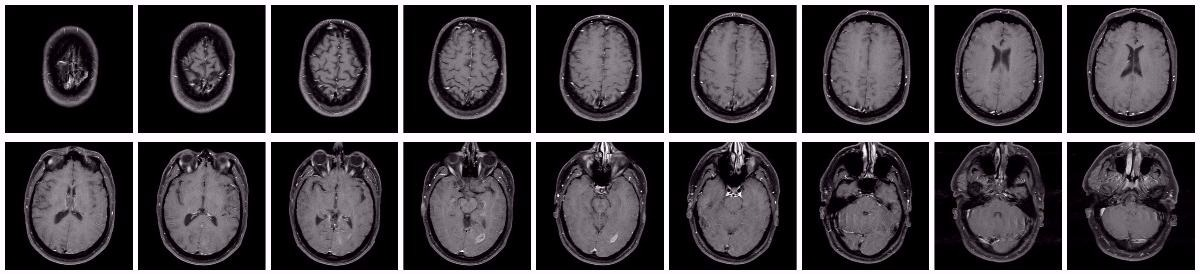
\includegraphics[width=15cm]{full-sequence}
 	\caption{Full Top-down Sequence of Individual}
 \end{figure}%
 
 
An entire sequence of scans is shown in Figure \ref{fig:full-sequence}.
In order to better determine the location within one single image and to improve the pattern matching performance, the images should b cropped to the skull in the middle of the image. Hence, the algorithm contained in the \textit{cropImages.py} file was developed that iterates over the \textit{x-axis} and \textit{y-axis} of each image and identifies the important parts of the image based on the brightness (see: secttion \ref{cv}). It's performance is vidualized in Figure \ref{fig:crop-image}. A new image is written to a file and used for the next processing step.

\begin{figure}
	\label{fig:crop-image}
	\centering
	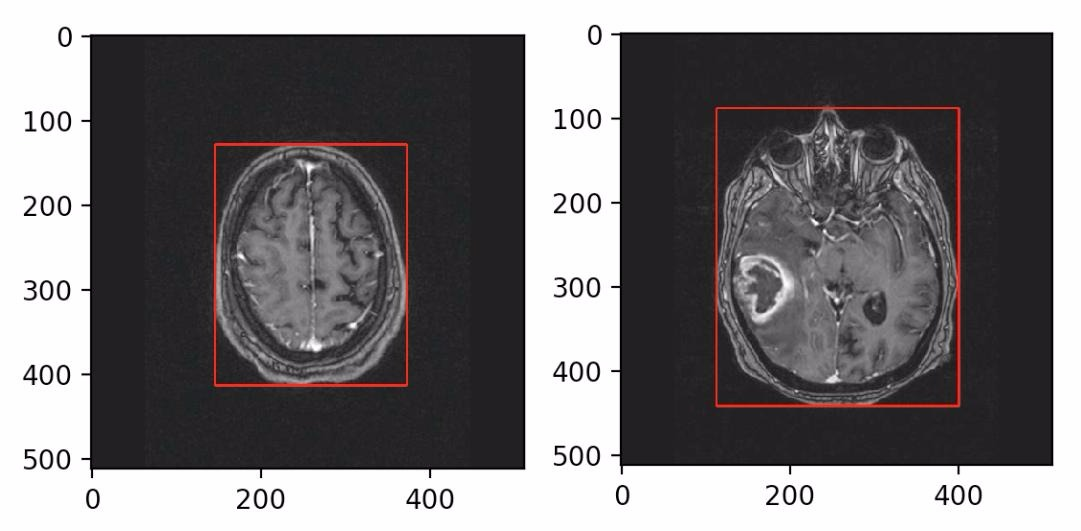
\includegraphics[height=4cm]{crop-image}
	\caption{Image Cropping}
\end{figure}%

\subsection{Pattern Matching}
After preprocessing the images, the main part of the algorithm that extracts features out of the image sequences for the following ML approach can be executed. The major idea of identifying a tumor within each image is based on a \textit{similarity measure} between a so-called \textit{template} and the \textit{target image}. For the actual matching, the \textit{OpenCV} library version \textit{2.4.13.2} for Python was used \citep{opencv}. 
In the following, I will explain the development of the matching template as well as the exact matching application.

\subsubsection{Template Development}
\label{template-dev}
To generate the template as an input for the matching process, I implemented an algorithm that develops a general pattern in form of an image that represents the average of a \textit{training image set}. As explain in section: \ref{cv}, a matrix can be used to represent each pixel of an image. Therefore, I manually selected some input tumor images and applied the algorithm provided in the \textit{generateTemplate.py} file. Each image is streched to the same size and to then calculate the average template matrix, the algorithm iterates over each pixel of each image and adds together all partial RGB values. This can be formulated as follows: 
\\

May $A_{j,k,c}^{i} \in \mathbb{N}$  and $0 < i < I , 0 < j < J , 0 < k < K , 0 < l < L $  
\\

where $I$ is the number of input pictures, 
$j$ is the number of  rows, 
$k$ is the number of columns and
$c$ refers to the color index.
Then, the average template image can be formulated as follows:
$$
\not\!\circ_{j,k,c} = \frac{\sum_{i=1}^{n} A_{j,k,c}^{i}}{I}
$$

$A^{i}$ can then be expressed as:
\[
(A)^{i}=
\begin{bmatrix}
a_{1,1} & a_{1,2} &  ... & a_{1,k}\\ 
a_{2,1} & a_{2,2} &  ... & a_{2,k}\\ 
... & ... & ... & ... \\ 
a_{j,1} & a_{j,2} & ... & a_{J,K}
\end{bmatrix}
\]
and  $a_{j,k} \in \mathbb{N}^{3}$ is refering to one pixel consisting of 3 color channels
\\


Figure \ref{fig:template-generation} demonstrates the input and result of this template creation process.

\begin{figure}
	\label{fig:template-generation}
	\centering
	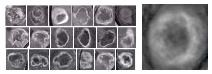
\includegraphics[height=4cm]{template-generation}
	\caption{Template Generation (left: input, right: output)}
\end{figure}%

\subsubsection{Matching Algorithm}
The core function of the data extraction from the input files is realized within the \textit{processImages.py} file. As mentioned before, OpenCV was used for matching the previously generated template (see: section \ref{template-dev}). The corresponding method in the OpenCV library is called \textit{cv2.matchTemplate()} and it basically slides the template image over the target image and computes how simililar it is to the current frame. The output is a new image in grayscale, where each pixel that ranges from 0 to 255 indicates how well the template matched the specific frame. It needs to be mentioned that depending on the chosen method, this result matrix can also be inverted meaning that the brightness can also indicate the output of the \textit{error term}.
As an argument, the function takes a specific method out of a set of six possible ones. Since all methods for creating the \textit{result matrix} are based on a similar mathematical approach, I want to discuss the best performing ones, which are called \textit{CV\_TM\_SQDIFF\_NORMED} and \textit{CV\_TM\_CCORR\_NORMED}. The underlying mathematical model for CV\_TM\_SQDIFF\_NORMED can be formulated as:

$$
R(x,y) = \frac{\sum_{x^{'},y^{'}}^{}(T(x^{'},y^{'})-I(x+x^{'},y+y^{'}))^2}{\sqrt{\sum_{x^{'},y^{'}}^{}T(x^{'},y^{'})^2}*\sum_{x^{'},y^{'}}^{}(I(x+x^{'},y+y^{'})}
$$

where $T$ is the template, which is matched to the Image $I$ resulting in the result of this metric. Hence, the value of $R$ at position $(x,y)$ refers to the goodness of the fit of $T$ on $I$ at this point. \\
The metric of CV\_TM\_CCORR\_NORMED is analogously defined as: 
$$
R(x,y) = \frac{\sum_{x^{'},y^{'}}^{}(T(x^{'},y^{'})*I(x+x^{'},y+y^{'}))^2}{\sqrt{\sum_{x^{'},y^{'}}^{}T(x^{'},y^{'})^2}*\sum_{x^{'},y^{'}}^{}(I(x+x^{'},y+y^{'})}
$$
\citep{opencvmethods}

Since the result matrix is also interpretable as an image, one can visually see the results of the matching algorithm. Figure \ref{fig:result-matrix} visualizes the result matrix for a given matching problem. The red square marks on the target image marks the corresponding position, which will be discussed again.

\begin{figure}
	\label{fig:result-matrix}
	\centering
	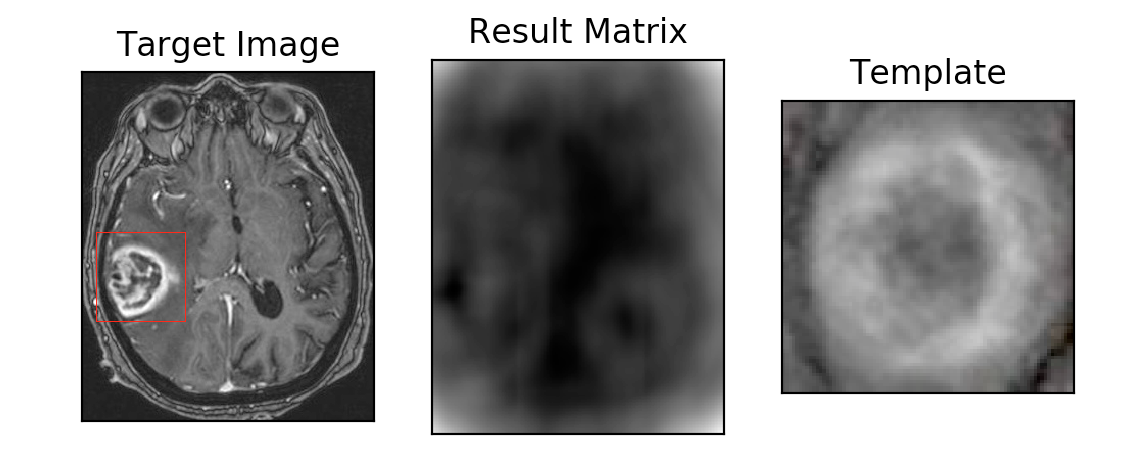
\includegraphics[height=5cm]{result-matrix}
	\caption{Target Image, Result Matrix and Template}
\end{figure}%

\subsubsection{Match Processing}
\label{ratio}
In this subsection, the focus is directed to the selection of the best match out of a sequence of images. When the result matrix for one image has been determined, it is required to further analyze the obtained result matrix in order compare it to the ones of other images. This is given by the fact, that a similar overall brightness level of the template favors a good match within an image sequence just due to the small distance in the color range. To overcome this problem, I invented a score that deals with this issue by computing a relative score for each retrieved result matrix. A specific characteristic of a good match is that the contrast between the matching position and its sorrpounding is quite high. This observation can be explained by the fact that the developed template his ring-shaped which lets it fit pretty well at a certain points but relatively bad in the area around it. To take advantage of this characteristic, the score basically evaluates the difference between the spot of the best matching point and the area. Hence, the template window size is taken around the matching point and a small circle is placed in the middle. This score, which can be uderstood as a ratio, can be formulated as follows:

	IConsider $X$ as the set of pixels within the template frame, where each $ w \in X $ is defined by its two coordinates $w=(x,y)$. The set of pixels within that inner circle with radius $R \in \mathbb{R} $ around the centre $w_{1} = (x_{1},y_{1})$ is defined as:
	$$ W_{1} = \{ (x,y) \in x: (x_{1} - x )^2+(y_{1} - y )^2 \leq R^2 \} $$ 
	The set of pixels around the circle is then 
	$$ W_{2} = X\setminus W_{1} $$
	
	Now, consider the function :
	$$h:X\xrightarrow[]{} [0, 255] \in \mathbb{N}  $$
	which maps each pixel to its brightness (the quality of the fit for this position). Then the total brightness of $K_{1} \in \mathbb{N} $ within the circle evaluates to:
	$$ K_{1} = \sum_{w_{1} \in W_{1}} h(w_{1})$$
	The total brigtness outside the circle is accordingly:
	$$ K_{2} = \sum_{w_{2} \in W_{2}} h(w_{2})$$
	Then, the final ratio $r$ can be computed as:
	$$ r = K_{1}\setminus K_{2} $$
	
	A visualization of this approach is shown in Figure \ref{fig:ratio}, where the ratio identifies the best matching image and position in the sequence.
	
	\begin{figure}
		\label{fig:ratio}
		\centering
		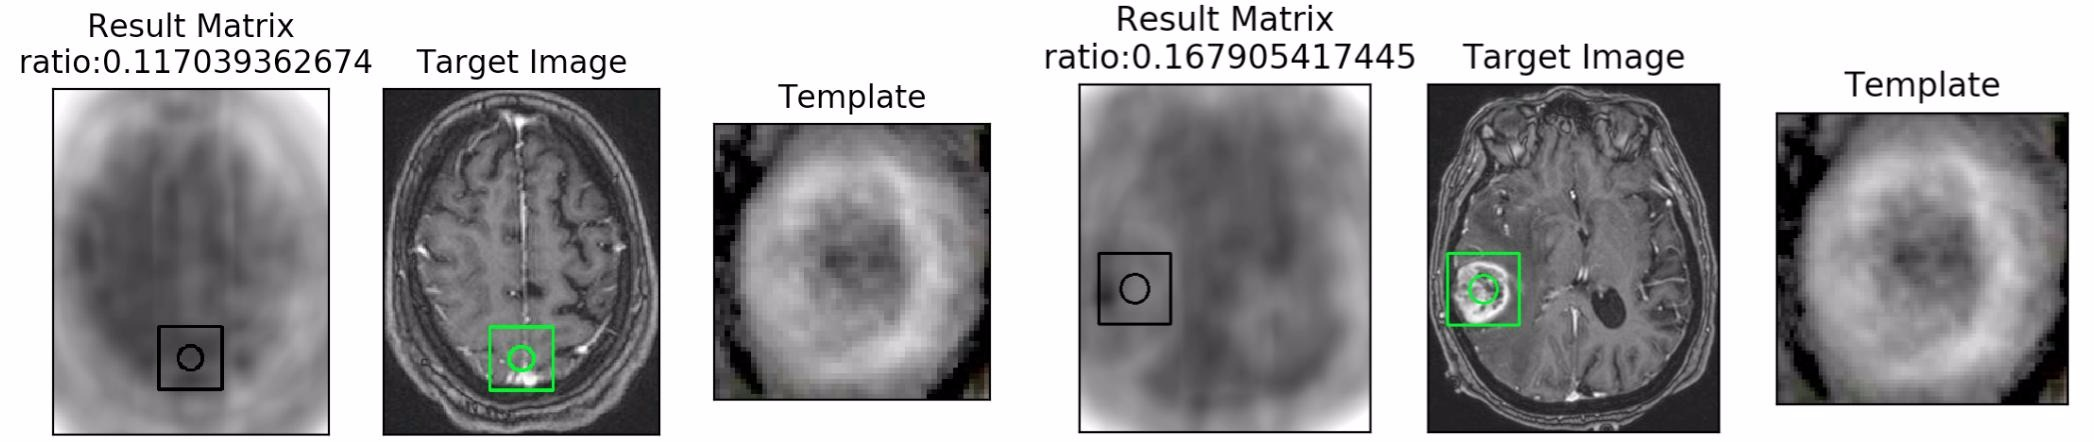
\includegraphics[height=4cm]{ratio}
		\caption{Application of Matching Ratio}
	\end{figure}%
	
	\subsubsection{Iteration steps and Output}
	At this point, I want to shortly describe the iteration of the algorithm in detail so that potential advancements and modifications can be considered easily. After the algorithm has computed the template image, it traverses the directory of images for each patients image sequence. For each image in the sequence the image is cropped and matched against the template. Here, two variables can be used to modify the execution:
	\begin{itemize}
		\item \textit{methods} is a list of all available methods within the pattern matching function of OpenCV, which can be added or removed from the list. However, for each method the execution is realized ones and the best match added to the output set.
		\item \textit{templateSizingSteps} is also a list that allows the programmer to specify the if the template should be resized to other proportions before matching. For each item in the list, the algorithm performs another execution and returns the best outcome.
	\end{itemize}
	
	The information that are gathered through the execution are written to the \textit{features.csv} file, where for each patient and each applied method the following information are persisted:
	
	\begin{itemize}
		\item \textit{relative position z} indicates in which image of the sequence with regard to the total number the bet match has been found.
		\item \textit{position y} determines the y coordinate of the position of the match
		\item \textit{position x} determines the x coordinate of the position of the match
		\item \textit{best probability} is the sum of all pixel values within the best matching template frame
		\item \textit{best probability ratio} is the value of relative probability score (see: section \ref{ratio}) 
	\end{itemize}
	
	Each row of this intermediate file is enriched with the most probable real tumor location. Since three radiologists were consulted for the evaluation of the tumor, the \textit{readTruthTable.py} file reads the provided information, evaluates the average of the provided expert opinions and returns them so that they can be written to the intermediate file.
	
\subsection{Classification}
	Within the previous sections, the comlex process of the information gathering was described, which is used as an input for the final classification task.
	
\bibliography{tumorDetection}
%\appendix
%\section*{Appendix A.}
%Some more details about those methods, so we can actually reproduce them.

\end{document}
